 %%%%%%%%%%%%%%%%%%%%%%%%%%%
 \newcommand{\documentName} { 2ª evaluación }
 \newcommand{\documentContent} { Global } 
 \newcommand{\waterMark} { Modelo A } 
 %%%%%%%%%%%%%%%%%%%%%%%%%%%
 
 % Configuración del documento.
 \newcommand{\schoolSubject} { Matemáticas 3º ESO - Recuperación}
\newcommand{\school} { IES La Serna }
\newcommand{\academicPeriod} { Curso 2020/2021 }


\newcommand{\autor} { Andrés Giménez Muñoz }
\newcommand{\emailAuthor} { agimenezmunoz@ieslaserna.com }
\newcommand{\autorSing}{ Profesores: Andrés } 
 \renewcommand{\schoolSubject} { Examen Matemáticas 2º ESO  }
\renewcommand{\school} { IES José de Churriguera  }
\renewcommand{\academicPeriod} { Curso 2022/2023 }

\renewcommand{\autor} { Andrés Giménez Muñoz }
\renewcommand{\emailAuthor} { andresprofemates@outlook.es }
\renewcommand{\autorSing}{ Profesor: Andrés } 
 
 % \renewcommand{\thepartno}{\arabic{partno}}
 \usepackage{nicefrac, xfrac}
 
 %%%%%%%%%%%%%%%%%%%%%%%%%%%
 % Exam configuration
 %\pointsdroppedatright   %% No mostrar la puntuación
 \pointsinrightmargin{} % Para poner las puntuaciones a la derecha. Se puede cambiar. Si se comenta, sale a la izquierda.
 \extrawidth{-1.5cm} %Un poquito más de margen por si ponemos textos largos.
 \marginpointname{ \emph{\points}}
 
 %% Si se comenta no aparecerán los espacios de la solución.
 %\nocancelspace
 
 %% Esto es de la clase exam. Si dejamos sin comentar \printanswers, se mostraran las soluciones. 
 %% Si la comentamos y dejamos sin comentar \noprintanswers, pues no se muestran las soluciones.
 % \printanswers
 %\noprintanswers
 
 %%%%%%%%%%%%%%%%%%%%%%%%%%%
 
 \begin{document}
 
 \StudentData{}
 \GradeTableHeader{}
 
 \justifying{}

 \justifying

\begin{center}
    \fbox{\fbox{\parbox{6.5in}{             
                \begin{itemize}
                    \item Deben aparecer todas las operaciones, no vale solo con indicar el resultado.
                    \item Se podrán quitar hasta cinco décimas por falta de claridad o rigor en el desarrollo de las respuestas o por una mala presentación.
                    \item No se puede utilizar la calculadora.
                \end{itemize}
            }}}
\end{center}
 
 \begin{questions}
    \question[1] Realiza las siguientes operaciones con números decimales:
    \begin {parts}
        \part $2,003 + 24,69 + 525,7$
        \vspace{\stretch{1}}

        \part $32,95 - 9,871$
        \vspace{\stretch{1}}

        \part $(5,2 - 6) \cdot 6$
        \vspace{\stretch{1}}
    \end{parts} 
    
    \question Divisiones 
    \begin {parts}
        \part [0\half] Realiza la siguiente división $34,95:3,1$ obteniendo dos decimales.
        \vspace{\stretch{2}} 

        \part [0\half] Haz la prueba de la división anterior.
        \vspace{\stretch{2}}
    \end{parts} 

    \newpage
    \question[1\half]Elisa ha hecho 43,5 kg de pasta y la quiere empaquetar en cajas de 0,250 kg.
    ¿Cuántas cajas necesita Elisa?
    \vspace{\stretch{1}}

    \question[1] Manuel compra 5 kg de tomates a 2,75 €/kg y paga con un billete de 20 €.
    \begin {parts}
        \part ¿Cuánto dinero se gasta?
        \vspace{\stretch{1}}
        \part ¿Cuánto le tienen que devolver? Redondea a una decima.
        \vspace{\stretch{1}}
    \end{parts} 

    \question[1]Realiza las siguientes operaciones con fracciones, simplificando el resultado al máximo:
    \begin {parts}
        \part $\frac{2}{3} + \frac{5}{9} + \frac{2}{4}$
        \vspace{\stretch{1}}
        
        \part $1 - \frac{2}{3} \cdot \frac{1}{5}$
        \vspace{\stretch{1}}

        \part $\frac{2}{5}: \frac{2}{3}$
        \vspace{\stretch{1}}
    \end{parts} 

    \question[1]Realiza las siguientes operaciones con fracciones, simplificando el resultado al máximo:
    \begin {parts}
        \part $\left(\frac{5}{4} - \frac{2}{3}\right) : \left(1 - \frac{4}{6}\right)$
        \vspace{\stretch{1}}
        
        \part $\frac{10}{7} \cdot \frac{21}{4} \cdot \frac{2}{5} $
        \vspace{\stretch{1}}
    \end{parts} 

    \newpage

    \question[1] Entre tres hermanos deben repartirse 120 \euro. 
    El primero se lleva $\frac{7}{15}$ del total, el segundo $\frac{5}{12}$ del total y el tercero el resto.
    \begin {parts}
        \part ¿Qué fracción del total se lleva el tercero?
        \vspace{\stretch{1}}
        \part ¿Cuánto dinero se ha llevado cada uno?
        \vspace{\stretch{1}}
    \end{parts} 

    \question[1] Un obrero gana 350 \euro a la semana. 
    ¿Cuánto gana en 45 días?
    \vspace{\stretch{2}}
    
    \question[1] Un coche tarda 45 minutos en recorrer 72 kilómetros. 
    ¿Qué distancia recorrerá en 3 horas si va a la misma velocidad?
    \vspace{\stretch{2}}

    \newpage

    \question[1] Una perfumería vende en una semana 57 frascos de una misma colonia. 
    Cada frasco lo vende a un precio de 8,35 \euro. 
    ¿Cuánto dinero ha recaudado por esta venta? 
    \vspace{\stretch{1}}

    \question[1] La perfumería ha recaudado 475,95\euro{} por la venta de una colonia y 1.368,70\euro{} por la venta de un perfume. 
    Si ha gastado 506,54\euro{} en electricidad ¿cuánto ha sido el beneficio total?
    \vspace{\stretch{1}}

    \newpage 
    \question[1] Ordena de menor a mayor los siguientes números: 
    \\
    $7,05$ \phantom{1234} $7,101$ \phantom{1234} $7,11$ \phantom{1234} $7,005$ \phantom{1234} $7,005$ \phantom{1234} $7,1$ \phantom{1234} $7$
    \vspace{\stretch{1}}
    
    \question[0\half] Obtén dos números decimales que estén comprendidos entre 8,2 y 8,3, uno que tenga dos decimales y otro que tenga tres.
    \vspace{\stretch{1}}

    \question[0\half] Sitúa en la recta, con precisión, los siguientes números decimales:
    \\ 
    $a=4,5$ \phantom{1234} $b=5,1$ \phantom{1234} $c=4,9$ \phantom{1234} $d=5,3$ \phantom{1234} $e=5,8$

    \vspace{2cm}

    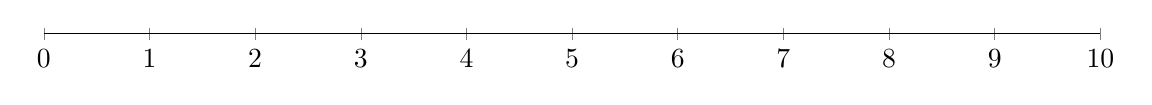
\begin{tikzpicture}
        % \begin{axis}[title = {Number line}, axis y line=none, y=0.5cm/3, restrict y to domain=0:50, axis lines=left]
        \begin{axis}[axis y line=none, y=0.6cm/3, restrict y to domain=0:50, axis lines=left,
            axis line style={-},
            width=15cm,
            xmax=10,ymax=10,xmin=0,ymin=-10]
        % \addplot+[only marks] coordinates  {( 3.14, 0 )( 10, 0 )}; 
        % \addplot+[only marks] coordinates  {( 20, 0 ) ( 21, 0 )}; 
        \end{axis}
        \end{tikzpicture}
    \vspace{\stretch{1}}
\end{questions}
 
\end{document}